%!TEX root = /Users/simo/Documents/PFC/Chapter1/chapter1.tex
\section{Especificaci\'on} % (fold)
\label{sec:especificacion}

Este proyecto surge de la necesidad de realizar presentaciones a distancia, mayoritariamente por videoconferencia. Las videoconferencias están en el día a día de las empresas, y dichas presentaciones suelen ir acompañadas de diferentes documentos, ya sean PowerPoint o PDF's. El realizar estas presentaciones a distancia genera una serie de problemas:

\begin{itemize}
	\item Cada \emph{usuario} ve el documento individualmente, por lo cual no hay una sincronía entre lo que todos ven. Cada uno puede estar mirando una hoja distinta, o a un punto distinto.
	\item A diferencia de en una presentación real, el ponente carece de una pizarra o una superficie donde hacer explicaciones cuando las diapositivas no son suficiente.
\end{itemize}

Estas dos carencias básicas hacen que se pierda un gran porcentaje del tiempo de dichas conferencias en \underline{forzar} esa sincronía, con explicaciones constantes de en qué diapositiva se está, o a qué punto mirar, o en simular dicha pizarra, con explicaciones verbales en vez de gráficas.

Este proyecto por tanto intenta ser una solución para dichas empresas (o cualquier usuario), de forma que se pueda disponer de ambas funcionalidades de forma sencilla y accesible. Se pretende explorar el mundo del desarrollo de aplicaciones web interactivas, profundizando en la comprensión de las capacidades de las tecnologías actuales, disponibles al público en los navegadores típicos.

\subsection{Limitaciones}
Considerando que el mayor uso de este software va a ser por parte de empresas u otras organizaciones, más que particulares, hace que se tengan que considerar una serie de limitaciones. Éstas son las básicas:

\begin{itemize}
	\item Las empresas generalmente no permiten instalar nuevo software en sus ordenadores.
	\item Hay que tener en cuenta que muchas empresas tienen instalados firewalls muy restrictivos.
	\item Los documentos no tienen porqué ser vistos por todo el mundo, debe de haber algún tipo de seguridad que permita que solo la gente adecuada pueda estar en la presentación.
\end{itemize}


\subsection{Funcionalidades}
Una vez definida los objetivos básicos que queremos alcanzar, y las restricciones, se pueden empezar a formalizar las funcionalidades. La solución más simple que cumpla las limitaciones, y que permita alcanzar dichas funcionalidades básicas, es la realización de una \textbf{web} que permita cargar documentos y dibujar sobre ellos de forma compartida con otros usuarios. Cualquier persona puede disponer de un explorador web, y generalmente funcionará a través del firewall. El tercer requisito se puede cumplir fácilemte, pues la seguridad web es un campo suficientemente desarrolado para ello. A continuación se numeran más detalladamente las funcionalidades que esta web ha de tener, separados en funcionalidades del sistema y de la pizarra en si.

\subsubsection{Funcionalidades del Sistema}
De entre las múltiples posibilidades a la hora de plantear el funcionamiento de la web, se ha considerado interesante estructurar la web como una ``comunidad'' en que, simplificando al máximo, los usuarios se registran, pueden subir sus documentos, e invitan a otros usuarios a que se unan a sus presentaciones. Por lo tanto:

\begin{description}
	\item[Gestión de Usuario] Se tiene que poder registrar, hacer login y salir. Todas las opciones tienen que ser modificables por el usuario, por ejemplo, la contraseña.
	\item[Gestión de Grupos] (Opcional) Poder crear grupos, invitar a usuarios a dichos grupos.
	\item[Gestión de Pizarras] Cada usuario tiene que poder crear sus pizarras (el concepto de pizarra y sus funcionalidades se detallan en la sección siguiente), editarlas, y eliminarlas. Tiene que poder invitar a otros usuarios y/o grupos a partizipar en esa pizarra.
	\item[Participación en otras Pizarras] Cada usuario tiene que poder ver las pizarras a las que ha sido invitado, acceder y salir de ellas. (Opcional) Rechazar y solicitar invitaciones.
\end{description}

\subsubsection{Funcionalidades de la Pizarra}
Se considera una pizarra como un lugar donde poder escribir, dibujar, al cual se le ha cargado unas imágenes de fondo, que se podrían considerar las diapositivas de una presentación. Una persona que tenga que hacer dos presentaciones a partir de dos archivos distintos, tendrá que crear dos pizarras distintas, e invitar a la gente adecuada. Se puede invitar a gente distinta en cada pizarra que se haya creado. La figura \ref{fig:concept1} es una representación básica de cómo se vería una pizarra en funcionamiento. Arriba habrían las herramientas de dibujo, y a la derecha la lista de usuarios conectados. Las funcionalidades deseadas para las pizarras son las siguientes:

\begin{figure}[ht]
\centering
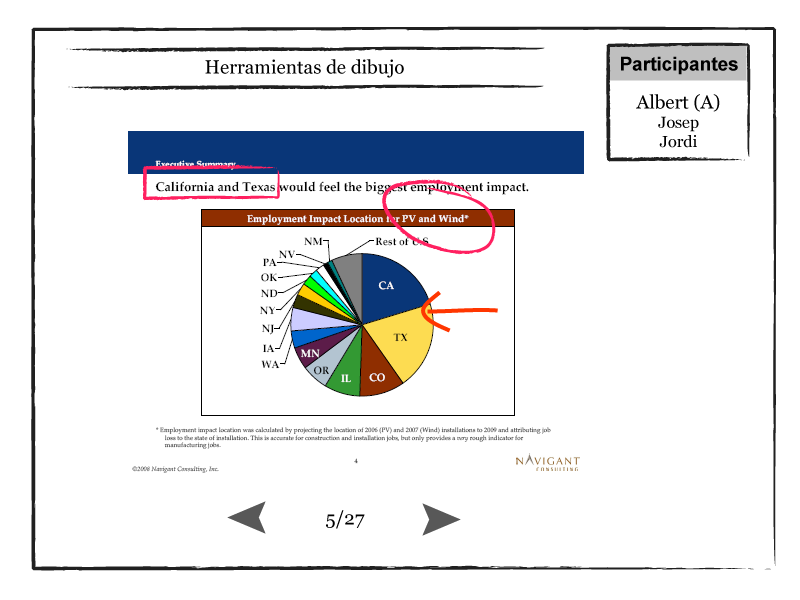
\includegraphics[width=16cm]{concepto.png}
\caption{Concepto básico de una pizarra}\label{fig:concept1}
\end{figure}

\begin{description}
	\item[Carga de documento] Cada pizarra tiene la posibilidad de añadir un documento que se cargará como imágenes de fondo. Dichas imágenes se pueden cargar de múltiples maneras.
	\begin{itemize}
		\item Una por una en formato de imagen JPG/PNG.
		\item Un zip/rar con el conjunto de imágenes.
		\item (Opcional) Mediante un PDF.
		\item (Opcional) Mediante una presentación PowerPoint directamente.
	\end{itemize}
	\item[Multipágina] Cada imagen tiene que ser una página diferente. Se tiene que poder avanzar y retroceder entre ellas.
	\item[Puntero] Se tiene que poder ver el puntero del ``administrador'', de forma que los usuarios pueden ver qué está señalando en ese momento, en vez de esperar a que dibuje un círculo, por ejemplo.
	\item[Herramientas de dibujo] Existen múltiples posibilidades para esto, y se intentarán implementar el máximo número posible, pero se establecen unos mínimos:
	\begin{description}
		\item[Lápiz] Con selección de color y grosor.
		\item[Lineas rectas] Con selección de color y grosor.
		\item[Texto] Con selección de color, fuente y tamaño. (Estos dos últimos opcionales)
		\item[Goma de borrar] Para poder eliminar objetos con la mayor sencillez posible.
		\item[Subrallador] (Opcional) Para todas las herramientas, poder seleccionar modo de subrallado, en que se harán los dibujos semitransparentes a modo de subrallador, en vez de sólidos.
		\item[Cajas y elipses] (Opcional)
		\item[Imágenes] (Opcional) Se desea la posibilidad de añadir imágenes extra, a parte de la del documento de fondo.
	\end{description}
	\item[Guardar] Se tiene que poder guardar la situación actual de la pizarra para cargarla posteriormente.
	\item[Formato en capas] (Opcional) Ya se entiende que cada pizarra tendrá dos capas, la de la imagen de fondo, y en la que se hagan todos los dibujos. Sería interesante hacer que se pueda dibujar por capas, crearlas, eliminarlas, moverlas arriba/abajo.
	\item[Exportar] Se tiene que poder exportar la situación de la pizarra en algun formato (pdf, imagen) y/o poder imprimirse.
	\item[Lista de usuarios] Listar los usuarios que están en ese momento conectados en la pizarra.
	\item[Chat] (Opcional) Posibilidad de establecer un chat entre los usuarios conectados. (Opcional) Poder guardar dicho chat junto con el estado de la pizarra.
\end{description}

\begin{figure}[h]
\centering
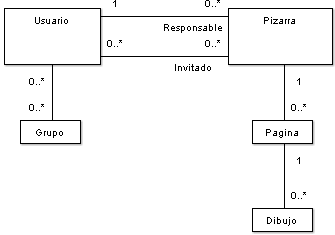
\includegraphics{Diagramadeclase1.png}
\caption{Diagrama de clases básico}\label{fig:diagramaclases}
\end{figure}

Para ayudar a entender el concepto de lo que será el sistema, la figura \ref{fig:diagramaclases} representa un diagrama de clases extremadamente simplificado.


\subsection{Tecnología}
Una explicación más detallada de la tecnología que se va a utilizar se podrá encontrar en las próximas secciones, pero hay una serie de requisitos que se afectan a la tecnología que se use, que deben ser considerados.

\begin{description}
	\item[Servidor] El servidor no tiene que requerir más de lo que sería un servidor web típico. Apache/MySQL sobre linux. Otros requisitos se admiten, pero tienen que estar accesibles de forma sencilla (binarios en forma de paquete, por ejemplo) para las distribuciones típicas de Linux. Nada de compilar fuentes, por ejemplo.
	\item[Cliente] Los navegadores más importantes tienen que estar soportados, Internet Explorer, Firefox y Safari como mínimo. Se intentará alcanzar el mayor grado de compatibilidad con Explorer 6, y en el peor caso, que cumpla las funcionalidades básicas.
	\item[Software] Puesto que los usuarios no tienen que tener que instalar ningún software nuevo, es altamente deseable que la web sea lo más sencilla posible. Se hará todo lo posible por evitar utilizar tecnologías que el usuario no tiene porqué tener instalados en su ordenador. Se va a intentar cumplir el requisito de que el usuario solo tiene que tener funcionando un navegador web moderno. En cuanto a la programación del esqueleto de la web, se considera interesante utilizar un lenguaje dinámico más moderno para agilizar el proceso, en vez del clásico PHP o ASP. También, el interés propio de explorar nuevas áreas, puesto que ya se tiene amplia experiencia con PHP, Ruby es un lenguaje muy interesante, y será considerado en la etapa de diseño.
\end{description}
